

\setchapterpreamble[u]{\margintoc}
\chapter{Electron spins, nuclear spins and their interaction}
\labch{electron_nuclear_interaction}

This chapter is dedicated to the description of the \Er electron spin and the nuclear spins in \Ca along with their interactions. The chapter will be organised as follows. \refsec{erbium_ions_in_ca} begins with the description of the energy levels of a Rare-Earth Ions (REIs) impurity in a crystal to arrive to an effective electron spin-1/2 approximation. This is followed in \refsec{nuclear_spins_ca} by a description of the nuclear spin Hamiltonian including the quadrupole interaction. Finally, the dipolar and exchange interactions between the different spin types are discussed in \refsec{interaction_between_to_spins}.

\section{Erbium ions in \Ca}
\labsec{erbium_ions_in_ca}

When placed in a crystalline host, $5s$ and $5p$ shells protect the energy-level structure of the unpaired electron. This allows one to treat the electrostatics of the crystal as a perturbation to the Free-Ion Hamiltonian. For ions with an odd number of electron spins\sidenote{\Er has 11 electron spins in its $4f$ shell.} the ground state will be a Kramers doublet. Consequently, when working at cryogenic temperatures, the ion can be effectively treated as an effective spin-1/2, as only the doublet is populated. We will now derive the spin-1/2 approximation from first principles.

\subsection{Free-ion Hamiltonian}

Given the protection of the erbium energy states to external perturbations, we consider first the energy level structure of the free \Er ion\sidenote{All details of the Free-Ion Hamiltonian can be found in \cite{weissbluth_atoms_2012, abragam_electron_2012}}. To describe the energy of an ion we consider the following Hamiltonian.

\begin{align}
\begin{split}
\mathcal{H}_{FI} &= \mathcal{H}_0 + \mathcal{H}_C + \mathcal{H}_{SO}, \\
\mathcal{H}_0 &= - \sum_{i=1}^N \frac{\hbar^2}{2m} \nabla_i^2 
- \sum_{i=1}^N \frac{Ze^2}{r_i}, \\
\mathcal{H}_C &= \sum_{i<j}^N \frac{e^2}{r_{ij}}, \\
\mathcal{H}_{SO} &= \sum_{i=1}^N \xi(r_i)\,\mathbf{l}_i \cdot \mathbf{s}_i.
\end{split}
\end{align}

Where $r_i$ is the distance of each electron to the nucleus and $r_{ij}$ are the distances between electrons. In order, the terms describe the kinetic and potential energy, the electron--electron Coulomb interaction and the spin--orbit coupling. For light ions, the spin--orbit coupling can be considered as a perturbation to the dominant electron--electron interaction. However, the Hamiltonian defined by the remaining terms cannot be directly solved, as it involves the coupling between $N$ independent electrons. This problem is solved by introducing the central-field approximation, where the electron--electron interaction is described with a single-electron potential averaged over all electron interactions. 

\begin{align}
\begin{split}
    \cH{FI} \approx& \cH{C} + \cH{NC} + \cH{SO}, \\
    \cH{C} =& \sum_{i=1}^N \frac{\hbar^2}{2m} \nabla_i^2  - \sum_{i=1}^N \frac{Ze^2}{r_i} + \left\langle\sum_{\text{pairs}} \frac{e^2}{r_{ij}}\right\rangle\\
    \cH{NC} =& \sum_{\text{pairs}} \frac{e^2}{r_{ij}} - \left\langle\sum_{\text{pairs}} \frac{e^2}{r_{ij}}\right\rangle
\end{split}
\end{align}

From this expression, it is clear that $\cH{NC}$ is merely a perturbation on $\cH{C}$. This allows to separate $\cH{0}$ into $N$ independent single-electron equations with the same angular properties as the Hydrogen atom. Each electron $i$ will be described by the four quantum numbers $(n, l, m_l, m_s)$, respectively the principal quantum number, the angular momentum quantum number ($0\leq l<n-1$), the magnetic quantum number ($-l\leq m_l\leq +l$) and the spin quantum number ($m_s=\pm\tfrac{1}{2}$). For lanthanides, the valence shell is located in the $n=4$ and $l=3$ configuration and is generally refered as the $4f$ shell \sidenote{The actual electronic wavefunctions are given by a Slater determinant, which enforces the Pauli exclusion principle and the anti-symmetric behaviour under electron exchange that is characteristic of fermionic particles.}. The averaged electron interaction term is not known, but it can be treated using the Hartree--Fock approximation (see \sidecite{weissbluth_atoms_2012}).

To calculate the effect of the non-central Hamiltonian $\cH{NC}$, the matrix elements of the Hamiltonian are calculated in a shared diagonal basis. This basis exploits the fact that both the angular momentum operators $\mathbf{L}$ and the spin operators $\mathbf{S}$ commute with $\cH{FI}$. This allows one to define a common basis with the set of eigenvectors of $\mathbf{L}^2$ and $\mathbf{S}^2$ (Russell--Saunders coupling).

Lastly, we consider the effects of the spin--orbit coupling on the energy structure. For light ions, with radially confined orbitals, this term is smaller than the rest of the interactions and can be treated as a perturbation. However, it is important to note that this term does not commute independently with $\mathbf{L}$ and $\mathbf{S}$ but with the combination of the two operators $\mathbf{J} = \mathbf{L} + \mathbf{S}$. Thus, the perturbation splits the degeneracy of the Russell--Saunders ground state into levels with a specific value of $J$, which are ($2J+1$)-degenerate. The labels are given by Russell--Saunders notation as $^{2S+1}L_J$\sidenote{Since erbium is a medium-sized ion, this approximation is not entirely valid, given that the spin--orbit coupling is no longer perturbative. Thus, $J$ and $S$ are no longer good quantum numbers, but remain relatively accurate for low-energy transitions.}. In the case of \Er, the free-ion ground state corresponds to $^4I_{15/2}$, a 16-fold degenerate level. The first excidecited level is separated by 1.5~\textmu m. In the following work, the \Ca crystal and the ions are cooled down to 10~mK. Consequently, only the ground state will be populated, which can be effectively approximated as a spin $J=15/2$.

\subsection{Crystal-field Hamiltonian}
When a lanthanide enters a crystal, it does so as a trivalent ion. Inside the crystal, the ion will be subject to the electrostatic field generated by the electronic clouds of the neighboring atoms. The crystal field breaks the spherical symmetry, which lifts the degeneracy of the free-ion states. However, the $4f$ electrons of a lanthanide are highly localized and shielded, so the crystal-field interaction can be treated as a perturbation to the free-ion energy levels. 

\begin{marginfigure}
    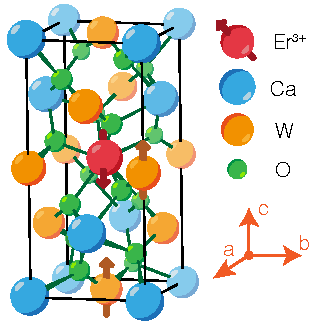
\includegraphics{chapter2/figures/crystal.pdf}
    \caption[\Ca crystal]{First unit cell of a \Ca crystall, centered around a substituting \Er ion.}
    \labfig{crystal}
\end{marginfigure}

We begin the section with a description of the host crystal. Calcium tungstate (\Ca), also known as scheelite, is a tetragonal crystal appearing as dipyramidal pseudo-octahedra and belongs to the $I4_1/a$ symmetry group. The crystal structure of \Ca\ consists of Ca$^{2+}$ and W$^{6+}$ ions coordinated by O$^{2-}$ ions. Each Ca$^{2+}$ ion is surrounded by eight O$^{2-}$ ions, forming a distorted dodecahedral environment, while each W$^{6+}$ ion is tetrahedrally coordinated by four O$^{2-}$ ions. The arrangement of these polyhedra leads to orthogonal principal axis (labeled as $a$, $b$ and $c$). Due to the symmetry of the crystal the $a$- and $b$- axis are equivalent. The unit cell parameters at cryogenic temperature are $a=b=5.23643$~\AA\,and $c=11.3381$~\AA\,\sidecite{senyshyn_lattice_2004}. 

Lanthanide ions enter the crystal in substitution to Ca$^{2+}$. Due to the difference in charge between the two ions, charge compensation mechanisms take place inside the crystal, which can be achieved by the presence of interstitial ions, vacancies, or other defects. Figure \reffig{crystal} shows an example of a \Ca crystal, where an \Er replaces the central calcium ion. The point symmetry of the \Er site is $S_4$, which notably lacks inversion symmetry. This has been shown to induce a magneto-optic effect which will be described in Section \ref{sec:magneto-optic}.

The crystal-field Hamiltonian is used to describe the interaction between the ion and the crystal and is generally described in terms of the extended Stevens operators $\hat{O}^q_k$ with $k=2,4,6,\dots$ and $q \in \{-k,\dots, k\}$ \sidecite{abragam_electron_2012,stevens_matrix_1952}

\begin{equation}
    \mathcal{H}_{\mathrm{CF}} = \sum_{k}^{2,4,6,\dots}\sum_{q}^{-k,...k} B_k^q \hat{O}^q_k \,
\end{equation}

\begin{margintable}
\centering
\begin{tabular}{l|l}
$B_2^0$    & 231~cm$^{-1}$  \\[-1em] \\ \hline \\[-1em]
$B_4^0$    & -90~cm$^{-1}$  \\[-1em] \\ \hline \\[-1em]
$B_4^4$    & 852~cm$^{-1}$  \\[-1em] \\ \hline \\[-1em]
$B_6^0$    & -0.6~cm$^{-1}$ \\[-1em] \\ \hline \\[-1em]
$B_6^4$    & 396~cm$^{-1}$  \\[-1em] \\ \hline \\[-1em]
$B_6^{-4}$ & 75~cm$^{-1}$  
\end{tabular}
\caption[Crystal field parameters]{Crystal field parameters for \Er:\Ca measured in \cite{enrique_optical_1971} with the operator normalization as defined in \cite{erath_crystal_1961}}
\label{tab:cf_parameters}
\end{margintable}

Where $B_k^q$ are the real-valued crystal field parameters. The extended Stevens operators are constructed as polynomial combinations of the $J_z$, $J_+$ and $J_-$ operators, and a full list of the operators can be found in \sidecite{altshuler_electron_1964}. The indices $k$ and $q$ encode the symmetry properties of the crystal field: $k$ specifies the rank of the operator (i.e., the maximum total power of angular momentum operators in the polynomial), and is restricted to even values due to time-reversal symmetry. The index $q$ determines the projection to the quantization axis (i.e. the maximum power of the non-diagonal terms). This allows the crystal field to encode the symmetry properties of the crystal site in a reduced number of terms. The values of the crystal-field parameters for \Er:\Ca are given in table \ref{tab:cf_parameters}. 

The effect of the crystal-field is the mixing of states with different $J$ and $J_z$, although the former is much weaker. For \Er, the 16-fold degenerate $^4I_{15/2}$ ground state is split into eight doublets ($Z_{1,\dots,8}$), known as \emph{Kramers doublets}. According to Kramers' theorem, \sidecite{kramers_general_1930} if the number of electrons in the $4f$ shell is odd and there is time-reversal symmetry (i.e. no magnetic field applied), then all crystal field levels are at least doubly degenerate, which is the case for \Er with $N=11$.

Each of the doublets can be modelled as an effective spin-1/2 with an anisotropic gyromagnetic factor that depends on the mixing between the $J_z$ wavefunctions. The energy difference between the $Z_1$ and $Z_2$ doublets is approximately 0.6~THz, which corresponds to a temperature of 50~K. At cryogenic temperatures (generally between 10~mK and 100~mK), only the $Z_1$ doublet will be populated, and the system can be effectively treated as an effective spin-1/2. During much of this work, this approximation will be used. Nevertheless, it is important to note that the application of a magnetic field can further mix the $J$-multiplet states, modifying the effective spin properties.

\begin{figure}
    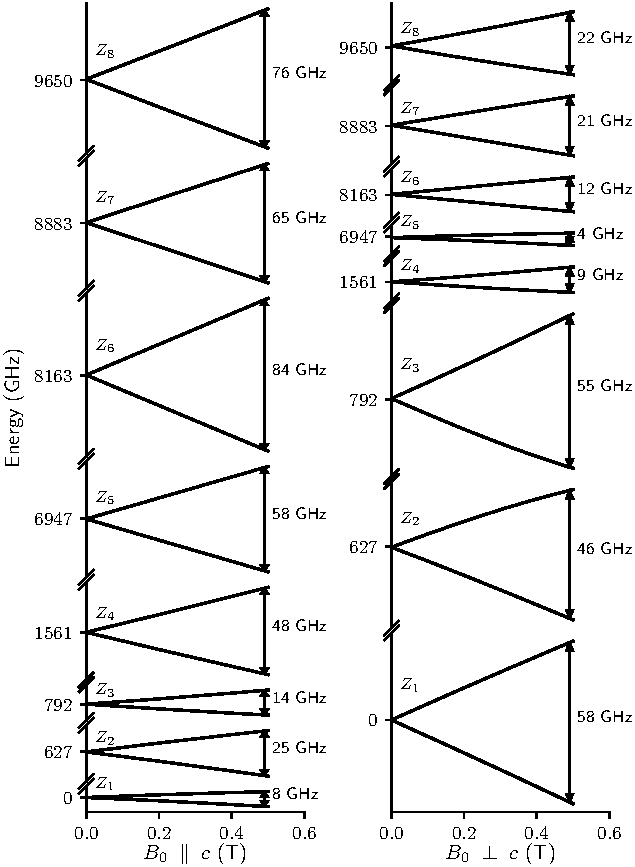
\includegraphics{chapter2/figures/energy_levels_vs_Bz_all.pdf}
    \caption[Crystal field levels]{Energy levels for all $Z_i$ doublets under a magnetic field parallel (perpendicular) to the $c$-axis. The y-axis is broken to better show the magnetic splitting of the levels. Energy difference between the states of each doublet at 500~mT is shown as vertical double arrows, along with the approximate frequency of the transitiion}
    \labfig{energy_levels_vs_Bz_all}
\end{figure}

Under a magnetic field $\mathbf{B_0}$, the Hamiltonian of the ground $J=15/2$-multiplet can be written as 

\begin{equation}
    \label{eq:J-CF_Hamiltonian}
    \mathcal{H}_J = \mu_B \ g_J\mathbf{B_0}\cdot \mathbf{J} + \mathcal{H}_{\mathrm{CF}},
\end{equation}

The first term represents the Zeeman interaction, where $\mu_B/2\pi = 13.996$~GHz/T is the Bohr magneton and $g_J = 6/5$ is the Landé factor for the \Er ground state. \reffig{energy_levels_vs_Bz_all} illustrates the magnetic-field-induced splitting of the energy levels along the $c$-axis, obtained by direct diagonalization of the Hamiltonian in Eq.~\ref{eq:J-CF_Hamiltonian}. Each $Z_i$ doublet splits into two levels, with an effective, anisotropic gyromagnetic tensor that varies for each doublet. This anisotropy is evident from the differing transition frequencies observed when a 500~mT magnetic field is applied parallel versus perpendicular to the $c$-axis. 

\subsection{Spin-1/2 approximation}

The energy separation between the $Z_1$ and $Z_2$ doublets is approximately 650 GHz, which corresponds to a temperature of 50~K. Thus, at the working temperature of 10~mK, only the $Z_1$ doublet will be populated. This doublet can be effectively treated as a spin-1/2 with an anisotropic gyromagnetic tensor,

\begin{marginfigure}
    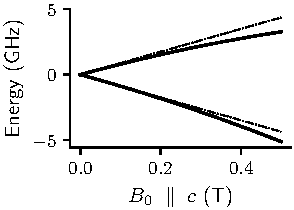
\includegraphics{chapter2/figures/energy_levels_vs_Bz_Z1.pdf}
    \caption[Zeeman splitting of the $Z_1$ doublet]{Energy levels of the $Z_1$ doublet as a function of magnetic field along the $c$-axis. The curves were obtaioned by direct diagonalization of Eq. \ref{eq:J-CF_Hamiltonian} and Eq. \ref{eq:er_spin_hamiltonian} (solid and dot-dashed resp.).}
    \labfig{energy_levels_vs_Bz_Z1}
\end{marginfigure}

\begin{equation}
    \label{eq:er_spin_hamiltonian}
    \mathcal{H}_S = \mathbf{B_0}\cdot \bar{\bar{\gamma}}_{^{3+}\text{Er}}\cdot\mathbf{S}
\end{equation}

with two eigenstates $\ket{\Downarrow}$ and $\ket{\Uparrow}$. The effective gyromagnetic tensor $\bar{\bar{\gamma}}_{^{3+}\text{Er}}$ is diagonal along the principal axes of the crystal, with values \sidecite{antipina.a._anisotropy_1981}

\begin{align}
\begin{split}
    \gamma_a = \gamma_b = \gamma_\perp &= -2\pi \times 117.3~\text{GHz/T}, \\
    \gamma_c = \gamma_\parallel &= -2\pi \times 17.45~\text{GHz/T}.
\end{split}
\end{align}

Throughout this thesis, we will primarily use this effective spin-1/2 approximation for the energy structure of the \Er. Nevertheless, it is important to note that as the magnetic field increases, mixing between doublets becomes significant, leading to deviations from the simple linear Zeeman splitting. This effect is illustrated in \reffig{energy_levels_vs_Bz_Z1}, where the energy levels of the $Z_1$ doublet are shown alongside the linear approximation as a function of magnetic field along the $c$-axis. Compared to the linear behaviour of the spin-1/2 approximation, the energy levels obtained from the crystal-field Hamiltonian "bend" as the magnetic field increases. A direct result of this non-linear behaviour is the appearance of a non-zero average magnetic moment

\begin{equation}
    \langle \mu_z \rangle = \frac{\partial E_\Downarrow}{\partial B_0} - \frac{\partial E_\Uparrow}{\partial B_0} \neq 0
\end{equation}

where $E_\Downarrow$ and $E_\Uparrow$ are the energies of the system as a function of the applied magnetic field $B_z$. This non-linearity is the origin of the pseudo-Zeeman \sidecite{baker_paramagnetic_1997} and pseudo-Quadrupole effects \sidecite{foley_secondorder_1947}, which are taken into account when interpreting the high-resolution spectroscopy experiments detailed in \red{labch}

\subsection{Magneto-Electric effect}
\label{sec:magneto-optic}

Paramagnetic impurities in non-centrosymmetric crystals exhibit a gyromagnetic tensor that depends on both the magnitude and orientation of an externally applied static electric field $\mathbf{E}$ \sidecite{ham_linear_1961}. This phenomenon is particularly strong in \Er:\Ca \sidecite{mims_electric_1965}, where it significantly influences the electron spin decoherence rate \sidecite{ledantec_twentythreemillisecond_2021}. The magneto-electric effect can be understood as a magnetically induced electric dipole. In Section \red{reference}, we perform NMR spectroscopy with high-resolution, and the effect of the dipole's electric field is key to understand one possible explanation to our observations. We follow with an explanation of this effect.

As noted earlier, \Er:\Ca occupies a site with $S_4$ symmetry, which lacks inversion symmetry. This allows odd terms $(k=1,3,5,\dots)$ to appear in the crystal-field Hamiltonian. These terms do not affect the ion's energy level structure in the absence of an external electric field and are not given in \reftab{cf_parameters}. The origin of these magneto-electric shifts lies in field-induced mixing between odd and even crystal-field terms which shifts the energy structure \sidecite{kiel_electricfieldinduced_1970}. This interaction can be modeled with the Hamiltonian:

\begin{equation}
    \mathcal{H}_{\text{m-e}} = \sum_{i,j,k}^{\{a,b,c\}} T_{k, i, j} S_{i} B_j E_k
\end{equation}

\begin{margintable}
\centering
\begin{tabular}{l|l|l}
param.         & value  & $S_4$ symm.   \\[-1em] \\ \hline \\[-1em]
$T_{a,c,a}$    & 1.4    & $-T_{b,c,b}$  \\[-1em] \\ \hline \\[-1em]
$T_{a,c,b}$    & 1.0    & $-T_{b,c,a}$  \\[-1em] \\ \hline \\[-1em]
$T_{c,a,a}$    & 5.4    & $-T_{c,b,b}$  \\[-1em] \\ \hline \\[-1em]
$T_{c,b,a}$    & 2.9    &  (-) 
\end{tabular}
\caption[Magneto-optic parameters]{Magneto-electric parameters for \Er:\Ca given in ($10^{-32} \times \frac{\text{J/T}}{\text{V/m}}$). The third column indicates the relation between the parameters that originate from the $S_4$ symmetry of the ion site. The rest of the values of the tensor can be obtained by enforcing $\{i, j\}$ index symmetry $T_{k, i, j} = T_{k, j, i}$.}
\labtab{magnetoelectric_parameters}
\end{margintable}

where $i,j,k \in\{x,y,z\}$ and $T_{k, i, j}$ is third-rank tensor which is symmetric in the {i, j} indices. The tensor captures the linear mixing of the levels as a function of the electric and magnetic field. The values for the tensor in \Er:\Ca were experimentally determined by Mims \sidecite{mims_electric_1965} and are displayed in \reftab{magnetoelectric_parameters}. The effect can be described with only four independent parameters and the rest of the elements of the tensor are obtained by enforcing $S_4$ and $\{i, j\}$ index symmetry.

Even if the energy shifts are zero in the absence of and electric field, this interaction can be understood as an induced electric dipole $\mathbf{d}$ due to an external magnetic field; if $\mathbf{B}$ is fixed, the interaction can be effectively rewritten as 

\begin{align}
\begin{split}
    \mathcal{H}_{\text{m-e}} &= \sum_k-d_k E_k = -\mathbf{d} \cdot \mathbf{E}, \\
    d_k &= - \sum_{i,j} T_{k, i, j} \langle S_{i}\rangle B_j.
\end{split}
\label{seq:electric_dipole}
\end{align}

where $\langle S_i \rangle$ corresponds to the expected value of the electron spin. The dipole in turn generates an electric field around the position of the \Er, whose effects will be revisited in \red{refsec}


\section[Nuclear spins in CaWO4]{Nuclear spins in \Ca}
\labsec{nuclear_spins_ca}

\subsection{Nuclear Zeeman interaction}

The coupling of a nuclear spin to a static magnetic field can be generally described with a nuclear Zeeman Hamiltonian

\begin{equation}
    \cH{nZ} = \gamma_n \mathbf{B_0}\cdot\mathbf{I},
\end{equation}

\noindent where $\gamma_n$ is the nuclear gyromagnetic ratio and $\mathbf{I}$ the nuclear spin operator which are inherent properties of a nucleus. The gyromagnetic ratio of a proton is $\gamma_p/2\pi = 42.57716$~MHz/T \red{ref} which is approximately 500 times smaller than the Bohr magneton. Given the large difference in magnetic response, the Zeeman energy of the electron spin is in general the dominating term in interacting systems. 

In addition, when the nuclear spin magnetic quantum number $I$ is larger than 1/2, the nuclear spin wavefunctions will not be spherical. Consequently, the charge distribution of the spin will be elongated and the pressence of an Electric Field Gradient (EFG) will introduce a new term in the Hamiltonian, known as the \textbf{quadrupole interaction}. We now proceed to derive the shape of the quadrupole Hamiltonian. 

\subsection{Electric Quadrupole interaction}
\labsec{electric_quadrupole}

%In section \red{labsec} we discuss the measurements performed in a system consisting of an \Er spin and a \Nb nuclear spin in close proximity. Although unexpected, the presence of a \Nb spin gave us the chance to study a more complex system, as it boasts a high nuclear spin $I=9/2$. This requires introducing the nuclear quadrupole interaction\sidenote{The quadrupole is strictly zero for $I=\tfrac12$}, which couples the nuclear electric quadrupole moment to the local electric-field gradient (EFG)

\begin{marginfigure}
    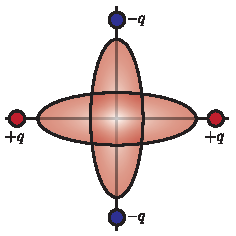
\includegraphics{chapter2/figures/charge_orientatons.pdf}
    \caption[Quadrupole charge diagram]{Non-spherical charge distribution with four charges, two $+q$ in the $x$-axis and two $-q$ in the $y$-axis. The positively charged distribution has two orientations: perpendicular and horizonatal. The perpendicular orientation is energetically more favourable.}
    \labfig{charge_orientatons}
\end{marginfigure}

Physically, the quadrupole effect arrises from the non-sphericity of the nuclear wavefunctions of $I\geq1$ nuclear spins. The charge distribution inside of the nuclear spin will be elongated and when subject to an external field gradient certain orientations of the charge will be favoured. \reffig{charge_orientatons} sketches this intuition by placing an elongated positively charged distribution between four charges, two $+q$ in the $x$-axis and two $-q$ in the $y$-axis. Due to the electrostatic attraction between the positive and negative charges, the vertical orientation will be energetically favoured.

We now proceed to sketch the derivation of the quadrupole interaction in terms of the spin operators which can be found in full in \sidecite{slichter_principles_1996}. We begin by considering the classical case of a charge distribution $\rho(\mathbf{r})$ under an electric potential $V(\mathbf{r})$. The energy associated to this system is given by

\begin{equation}
    E = \int \rho(\mathbf{r}) \times V(\mathbf{r}) d\mathcal{V}.
\end{equation}

We can approach this problem through the multi-pole expansion, which consists on writing the potential as a Taylor series at the center of mass of the nucleus and treating each term independently, 

\begin{equation}
V(\mathbf{r}) = V(0) 
+ \sum_{\alpha} x_{\alpha} 
\left. \frac{\partial V}{\partial x_{\alpha}} \right|_{\mathbf{r}=0}
+ \frac{1}{2!} \sum_{\alpha,\beta} x_{\alpha} x_{\beta} 
\left. \frac{\partial^2 V}{\partial x_{\alpha} \partial x_{\beta}} \right|_{\mathbf{r}=0}
+ \cdots
\end{equation}

Consequently, the energy will be written as \sidenote{We have introduced the notation \[V_{\alpha}=\frac{\partial V}{\partial x_{\alpha}}, \quad V_{\alpha \beta}\equiv\frac{\partial^2 V}{\partial x_{\alpha} \partial x_{\beta}},\] \noindent which correspond to the electric field and the EFG respectively.}

\begin{align}
\begin{split}
E =&\, V(0) \int \rho \, d\mathcal{V} 
+ \sum_{\alpha} V_{\alpha} \int x_{\alpha} \rho \, d\mathcal{V} +\\
+&\, \frac{1}{2!} \sum_{\alpha,\beta} V_{\alpha \beta} \int x_{\alpha} x_{\beta} \rho \, d\mathcal{V} 
+ \cdots
\end{split}
\end{align}

Respectively, each term corresponds to the electrostatic energy of a point-charge nucleus, the energy due to the dipole moment \sidenote{Given that the center of mass and the center of charge are equal, the dipole energy tends to zero} and the quadrupolar term. To describe the quadrupole interaction, it is particularly useful to introduce the following quantities 

\begin{equation}
    Q_{\alpha \beta} = \int \big( 3 x_{\alpha} x_{\beta} - \delta_{\alpha \beta} r^{2} \big) \, \rho \, d\mathcal{V}
\end{equation}

as the energy of the quadrupole can be written in a compact form

\begin{equation}
    E_\text{Q} = \tfrac16 \sum_{\alpha, \beta} Q_{\alpha \beta} V_{\alpha \beta}.
\end{equation}

To quantize this expression one must take the quantum mechanical expression for the charge density of the constituting protons of the nucleus and apply the Wigner-Eckart theorem to evaluate the resulting integrals and express the interaction in terms of the nuclear spin operator $\mathbf{I}$ 

\begin{equation}
\cH{Q} = \frac{e\mathcal{Q}}{6I(2I-1)} 
\sum_{\alpha,\beta} V_{\alpha\beta} 
\left[ \tfrac{3}{2} \left( I_{\alpha} I_{\beta} + I_{\beta} I_{\alpha} \right) 
- \delta_{\alpha\beta} I^{2} \right].
\label{eq:quadrupole}
\end{equation}

where $\mathcal{Q}$ denotes the quadrupole moment, obtained from the integral of the nuclear charge distribution and measured in Barns. The quadrupole Hamiltonian can be writen the following compact form

\begin{equation}
    \cH{Q} = \mathbf{I} \cdot \bar{\bar{Q}} \cdot \mathbf{I},
\end{equation}

\noindent where $\bar{\bar{Q}}$ is the quadrupole tensor, proportional to the EFG. The EFG satisfies Laplace's equation, so its components obey $V_{xx}+V_{yy}+V_{zz}=0$, and by electrostatic symmetry $V_{\alpha\beta}=V_{\beta\alpha}$. Consequently, the EFG (and thus $\bar{\bar{Q}}$) is a real, symmetric, traceless rank-2 tensor and can be diagonalized. In the principal-axis frame $(\mathcal{P}_1,\mathcal{P}_2,\mathcal{P}_3)$, choosing the $\mathcal{P}_1$ axis so that $|V_{11}|\ge|V_{22}|\ge|V_{33}|$, one defines the conventional asymmetry parameter

\begin{equation}
    \eta = \frac{V_{33}-V_{22}}{V_{11}}, \qquad 0\leq\eta\leq1,
\end{equation}

\noindent and the Hamiltonian in the principal-axis system can be expressed as

\begin{equation}
\cH{Q} = \frac{\hbar \omega_Q}{6}\left[ 3 I_{\mathcal{P}_1}^2 - I(I+1) + \eta(I_{\mathcal{P}_2}^2 - I_{\mathcal{P}_3}^2)\right],
\label{eq:quadrupole_ppaxis}
\end{equation}

where $\hbar \omega_Q$ is the quadrupole energy,

\begin{equation}
    \omega_Q \equiv  \frac{3e\mathcal{Q}V_{11}}{2I(2I-1)\hbar}.
\end{equation}

Based on the value of the asymmetry parameter $\eta$ we can distinguish two regimes. First, if $\eta=0$ the quadrupole is said to be axial and the Hamiltonian is diagonal in the $\ket{I,m_I}$ basis. The quadrupole then splits the nuclear energy levels by $m_I^2 \omega_Q/2 $, where $m_I$ is the projection of the nuclear spin along the $\mathcal{P}_1$ axis. Second, when $\eta\neq0$ the term proportional to $\eta$ mixes states differing by $\Delta m_I=\pm2$ and creates a non-trivial energy level structure. 


\subsubsection{Rotational invariance of the quadrupolar energy spectrum}

When measuring the nuclear spin transitions under a specific magnetic field orientation, the resulting frequencies are generally not enough to describe the full quadrupole tensor. 

It is useful to express the quadrupole in the basis of the rank-2 spherical tensors\sidenote{
The rank-2 spherical tensors are related to the spin operator basis by
\begin{equation*}
\begin{split}
T^{(2)}_{0} &= 3 I_z^2 - I(I+1), \\
T^{(2)}_{\pm 1} &= \mp \left( I_z I_{\pm} + I_{\pm} I_z \right), \\
T^{(2)}_{\pm 2} &= I_{\pm}^2 .
\end{split}
\end{equation*}
}. By algebraic manipulation of Eq. \ref{eq:quadrupole} we can rewrite the Hamiltonian as

\begin{equation}
    \cH{Q} = \sum_{m = -2}^2 Q_m T^{(2)}_m(\mathbf{I})
    \label{eq:quadrupole_spherical}
\end{equation}

\noindent with

\begin{equation}
\begin{aligned}
Q_{0} &= Q_{zz}, \\
Q_{\pm 1} &= Q_{zx} \pm i Q_{zy}, \\
Q_{\pm 2} &= \tfrac{1}{2}(Q_{xx} - Q_{yy}) \pm i Q_{xy}.
\end{aligned}
\end{equation}

One can show (Appendix \ref{app:rotations_quadrupole}) that the coefficients transform as 
\begin{equation}
Q_m \;\mapsto\; e^{-im\zeta}\, Q_m,
\end{equation}
under a physical rotation of angle $\zeta$ about the $z$-axis. Since the energy levels of the Hamiltonian are insensitive to these phase factors and depend only on invariants such as $Q_0$, $|Q_{\pm 1}|^2$, and $|Q_{\pm 2}|^2$, the energy spectrum is invariant under such rotations. 

This is a subtle point with an important consequence: any two tensors related by a rotation in the $xy$ plane produce identical NMR spectra for a fixed field orientation. Equivalently, no matter how precise the measurement of the nuclear transition frequencies, one can reconstruct the quadrupole tensor only up to a rotation about the field axis. Consequently, the only way to lift this degeneracy is by measuring with a different quantization axis of the nuclear spin\sidenote{At zero magnetic field, no orientation information can be extracted, only the magnitudes of the principal components of the quadrupole}.

\subsection{Magnetic spin environment}

The nuclear spin environment of \Ca is predominantly composed of \W nuclear spins, which have a natural abundance of 14.4\% and remarkably low gyromagnetic ratio\sidenote{It is 0.041 times smaller than the proton's gryomagnetic factor!}, $\gamma_{\text{\W}}/2\pi = 1.77394$~MHz/T \sidecite{knight_solidstate_1986}. The combination of a low density of nuclear spins and a weak gyromagnetic ratio results in an environment with a reduced magnetic moment density.
\sidenote{There are other stable calcium and oxygen isotopes with non-zero nuclear spin, namely $^{43}$Ca, $^{15}$O and $^{17}$O with $I=7/2$, $I=1/2$ and $I=5/2$, respectively, but their natural abundances are low (0.1\%, 0.003\% and <0.003\%, respectively) and are not considered in our discussion.}
As such, the magnetic noise perceived by any paramagnetic impurity hosted in the crystal is significantly reduced compared to other hosts used in quantum applications, such as yttrium orthosilicate (Y$_2$SiO$_5$, YSO) and yttrium oxide (Y$_2$O$_3$). This results in slow spectral diffusion and reduced decoherence rates for any paramagnetic impurity hosted in the crystal.

In addition to the nuclear spin bath, paramagnetic impurities—such as other rare-earth ions or transition metal ions—can also contribute significantly to the magnetic environment experienced by a single \Er ion. These electronic spins have a much larger gyromagnetic response and are more spatially delocalized than the point-like nuclear spins. At high concentrations, the magnetic noise is dominated by the paramagnetic impurities rather than the nuclear bath. Therefore, minimizing the dopant concentration is crucial to achieve long coherence times. Indeed, by reducing the concentration of rare-earth ions to the 1--100 parts per billion (ppb) range and exploiting the low magnetic density, ensemble spin coherence times as long as 23~ms have been demonstrated for \Er:\Ca \sidecite{ledantec_twentythreemillisecond_2021}.

The sample used for this work was grown using high-purity, natural-abundance materials and no paramagnetic impurities were added during crystal growth\sidenote{Specific details on the growth of a similar sample can be found in \cite{erb_growth_2013}.}. Nevertheless, trace amounts in the precursors result in a concentration of \Er of 3.1~ppb, measured using electron spin resonance (ESR) techniques \red{appendix}. There are four calcium sites in a single unit cell with volume $V_{\text{unit cell}}\sim310\ \text{\AA}^3$. This results in in average distance between ions of 0.3 \textmu m. \sidenote{The Ca site density is 
\begin{equation*}
    4/310 \approx 1.3\times10^{-2} \text{~A}^{-3}
\end{equation*} 
With [\Er]=3.1~ppb, the \Er density is 
\begin{equation*}
    n_{\text{\Er}} \approx 4.0\times10^{-11} \text{~A}^{-3}
\end{equation*} 
and the characteristic spacing is
\begin{equation*}
    n_{\text{\Er}}^{-1/3} \approx 2.9\times10^{3}\text{~A}\approx0.29\text{~\textmu m} 
\end{equation*}
} 
This distance is large enough that interactions between paramagnetic impurities can be effectively neglected except in specific cases where two ions are, by chance, in close proximity. Consequently, we consider that the magnetic environment in the crystal is dominated by \W nuclear spin.

\section{Interaction between two spins}
\labsec{interaction_between_to_spins}

In this thesis, individual \Er ions in \Ca are used as a ancilla spins to address individual nuclear spins in their vecinity. We now proceed to consider the interaction between the two spin species which is mainly dominated via the long-range dipolar interaction\sidenote{
    We do not consider exchange interaction between the electron and nuclear spins. The \Er and W ions in the crystal are coordinated by an oxygen ion (see \labfig{crystal}) which prevents direct overlap between the spin wavefunctions. 
}.

The magnetic interaction between two dipoles with magnetic vector moments $\boldsymbol{\mu}_1$ and $\boldsymbol{\mu}_2$ is expressed as\sidecite{abragam_electron_2012}

\begin{equation}
    \mathcal{H}_{dd} = \frac{\mu_0}{4\pi} r^{-3} 
    \left[ \boldsymbol{\mu}_1 \cdot \boldsymbol{\mu}_2 
    - 3r^{-2} (\boldsymbol{\mu}_1 \cdot \mathbf{r})(\boldsymbol{\mu}_2 \cdot \mathbf{r}), \right]
\end{equation}

\noindent where $\mathbf{r}$ is the vector separating the two spins. In the case of \Er and a neighboring nuclear spin $\boldsymbol{\mu}_1 = \bar{\bar{\gamma}}_{^{3+}\text{Er}} \cdot \mathbf{S}$ and $\boldsymbol{\mu}_2 = \gamma_n \mathbf{I}$. Expanding the expression in terms of the spin operators yields

\begin{equation}
\begin{aligned}
H_\text{hf} &= 
\frac{\mu_0 \gamma_\text{\W}}{4\pi r^3} \Big[ 
\gamma_{\perp} S_{a} I_{a} \big( 1 - 3 \sin^2 \theta_r \cos^2 \phi_r \big) \\
&\quad + \gamma_{\perp} S_{b} I_{b} \big( 1 - 3 \sin^2 \theta_r \sin^2 \phi_r \big) \\
&\quad + \gamma_{\parallel} S_{c} I_{c} \big( 1 - 3 \cos^2 \theta_r \big) \\
&\quad - 3 \sin^2 \theta_r \cos \phi_r \sin \phi_r 
\big( \gamma_{\perp} S_{a} I_{b} + \gamma_{\perp} S_{b} I_{a} \big) \\
&\quad - 3 \sin \theta_r \cos \phi_r \cos \theta_r 
\big( \gamma_{\perp} S_{a} I_{c} + \gamma_{\parallel} S_{c} I_{a} \big) \\
&\quad - 3 \sin \theta_r \sin \phi_r \cos \theta_r 
\big( \gamma_{\perp} S_{b} I_{c} + \gamma_{\parallel} S_{c} I_{b} \big) 
\Big].
\end{aligned}
\end{equation}

\noindent where $\theta_r$ and $\phi_r$ are, respectively, the polar and azimuthal angles of the vector $\mathbf{r}$ and the spin operators are expressed in the crystal axis basis. This interaction can be written in a more compact form:

\begin{equation}
    \cH{d-d} = \mathbf{S} \cdot \bar{\bar {A}} \cdot \mathbf{I},
\end{equation}

\noindent where the complexity of the dipolar interaction is encoded in the hyperfine tensor $\bar{\bar{A}}$. This interaction is strongly anisotropic and depends on the relative position and orientation between the two spins. In line with the experimental conditions discussed later, we take the magnetic field to be approximately parallel to the $c$-axis of the crystal.Therefore, their coupling will depend on the orientation of the external magnetic field. In the high-field regime\sidenote{This corresponds to
\begin{equation*}
|\bar{\bar{\gamma}}_{^{3+}\text{Er}} \cdot \mathbf{B_0}| \gg \bar{\bar A}.
\end{equation*}
If the separation between the spins is $a$, the condition can be approximated as
\begin{equation*}
|\mathbf{B_0}| \gg \frac{\gamma_{\text{\W}} \mu_0}{ 8\pi a^3} \approx 1\text{~mT}.
\end{equation*}} the dominant term in the Hamiltonian is the Zeeman energy of \Er and non-commuting terms can be treated as perturbations to the energy-level structure. In particular, hyperfine interaction terms involving $S_x$ and $S_y$ can be disregarded in what is known as the secular approximation. The resulting Hamiltonian is given by\sidenote{}

\begin{align}
\begin{split}
    \cH{d-d} \approx A_\perp I_x + A_\parallel I_z,
\end{split}
\end{align}

\noindent where the $x$-axis has been chosen to be parallel to the direction of the perpendicular hyperfine coupling.

Intuitively, the secular approximation can be understood by considering the effects of each term in the \Er spin Bloch sphere. The dominant Zeeman term induces a precession of the electron spin around the $z$-axis with frequency $\gamma_\parallel B_0$. By contrast, the hyperfine terms involving $S_x$ and $S_y$ correspond to rotations around the $x$- and $y$-axes, with much smaller frequencies. Because of the large difference in frequency scales, the transverse rotations effectively average to zero and can be neglected.

\begin{figure}
    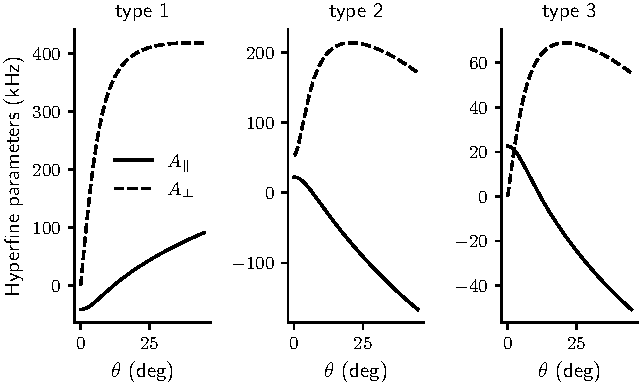
\includegraphics{chapter2/figures/hyperfine_tensor_vs_angle.pdf}
    \caption[Hyperfine coupling parameter]{Parallel and perpendicular hyperfine couplings as a function of the angle $\theta$ between the magnetic field $B_0$ and the $c$-axis of the crystal for the three types of W-sites.}
    \labfig{hyperfine_tensor_vs_angle}
\end{figure}


\begin{margintable}[]
\begin{tabular}{l|l}
       & distance (\AA) \\ \hline
type 1 & $(+2.62, +2.62,  0) $           \\
       & $(+2.62, -2.62,  0)  $          \\
       & $(-2.62, +2.62,  0)$            \\
       & $(-2.62, -2.62,  0)$            \\ \hline
type 2 & $(+2.62,  0, -2.84)$            \\
       & $(-2.62,  0, -2.84)$            \\
       & $(0, +2.62, +2.84)$             \\
       & $(0, -2.62, +2.84)$             \\ \hline
type 3 & $(0, 0, +5.69)$                 \\
       & $(0, 0, -5.69)$                
\end{tabular}
\caption[\W atomic positions]{W site positions in \Ca, separated in three types depending on their relative position to the central \Er ion}
\labtab{w_positions}
\end{margintable}

Within the first unit cell, and with $B_0$ applied parallel to the $c$-axis, three sets of magnetically-equivalent \W atoms can be found, called types 1, 2, and 3 in the following. All \W nuclear spins beyond the first unit cell have lower couplings and are not resolved in this work. Table \reftab{w_positions} indicates the atomic positions of the ten W-sites within a unit cell centered around an \Er ion. The value of the hyperfine parameters $A_\parallel$ and $A_\perp$ are plot as a function of the angle between the applied magnetic field and the $c$-axis is \reffig{hyperfine_tensor_vs_angle}. The strong dependence of the hyperfine coupling with the angle evidences the anisotropic nature of the interaction, with values that can change from a zero to hundreds of kHz in less than 10º.

We can also consider the interaction between two \W nuclear spins. Since both spins are have an isotropic gyromagnetic factor, they will both be aligned to the externally applied field in the high field regime. For the two aligned spins the interaction is then simplified to

\begin{equation}
    \cH{d-d} = \frac{\mu_0\gamma_{\text{\W}}^2}{4\pi r^3}  \mathbf{I_1} \mathbf{I_2} \left[ 1 - 3\cos(\theta_r) \right],
\end{equation}

\noindent and the average strength of the interaction is

\begin{equation}
    \frac{\mu_0\gamma_{\text{\W}}^2}{8\pi a^3} \approx 1\text{~Hz}, 
\end{equation} 

\noindent which is orders of magnitude smaller than the \Er-\W coupling and Zeeman terms. Therefore, the nuclear spin bath interactions will be slow compared to the dynamics of the paramagnetic ion and the neighbouring nuclear spins.

%\subsection{Exchange interaction}

%The exchange interaction, also known as Fermi-contact interaction, takes the following form \sidecite{abragam_electron_2012}:

%\begin{equation}
%    \cH{exch} = \mathbf{S_1} \cdot \bar{\bar {J}}_\text{exch} \cdot \mathbf{S_2}
%\end{equation}

%Contact interactions only occur when the spin wavefunctions overlap with each other and the typical interaction range is $\sim$1.5~nm \sidecite{schweiger_principles_2001}. We do not consider contact interactions between two nuclear spins as the wavefunctions are almost point-like.

%The wavefunctions of \Er ions are highly localized thanks to the $5s$ and $5p$ shielding. Additionally, thanks to the low density of \Er ions we can discard any possible contact term between two distant electron spins. 

%In the case of electron and nuclear spin interaction, the \Er and W ions in the crystal are coordinated by an oxygen ion (see \labfig{crystal}) which prevents direct overlap between the spin wavefunctions. We conclude that contact interaction between proximal \Er ions and \W nuclear spins is not the primary coupling; at most they may produce small isotropic shifts.

%We conclude that the dominating interaction mechanism between two spins in our system is the free-space dipolar coupling.

\section{\W-\Er Hamiltonian}
\labsec{w_er_hamiltonian}

We now consider the Hamiltonian of an \Er spin-1/2 coupled via hyperfine interaction to a nuclear spin-1/2 while under a magnetic field $B_0$. As described in this chapter, the Hamiltonian will be

\begin{equation}
    \cH{}/\hbar = \omega_S \hat{S}_z + \omega_I \hat{I}_z + A_\parallel \hat{S}_z \hat{I}_z + A_\perp \hat{S}_z \hat{I}_x.
\end{equation}

We remark that the $S_z$ and $I_z$ operators should be understood as the electron and nuclear spin quantization axis respectively. For the case of the isotropic nuclear spin, this axis is parallel $\mathbf{B_0}$, but the quantization axis of the electron spin differs from the applied magnetic field direction due to its anisotropic gyromagnetic tensor (see \reffig{energy_levels_half_v2}a).

This Hamiltonian defines a four-level system and can be analytically solved \sidecite{schweiger_principles_2001}. The resulting energy levels of the system can be described as an admixture of the uncoupled spin states $\ket{\Downarrow \uparrow}$, $\ket{\Downarrow \downarrow}$, $\ket{\Uparrow \uparrow}$, $\ket{\Uparrow \downarrow}$: 


\begin{figure}
    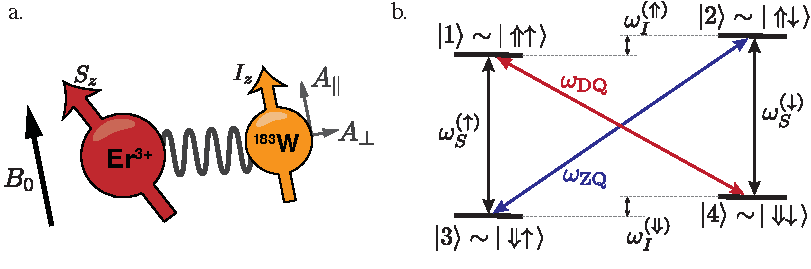
\includegraphics{chapter2/figures/energy_levels_half_v2.pdf}
    \caption[\W-\Er coupled system]{
        \textbf{a.} \W-\Er coupled system. The \Er spin (red) interacts with a \W spin (orange) through the hyperfine interaction (gray). The quantization axis of the spins $S_z$ and $I_z$ differ from each other due to the anisotropy of the \Er gyromagnetic tensor.
        \textbf{b.} Energy level diagram of the coupled system in the high field regime approximation. Allowed EPR transitions are shown with a black arrow while zero-quantum and double-quantum transitions are shown with blue and red arrows respectively.}
    \labfig{energy_levels_half_v2}
\end{figure}


\begin{align}
\begin{split}
    \ket{1} &= \cos\left(\tfrac{\eta_{\Uparrow}}{2}\right) \ket{\Uparrow\uparrow} 
                 - \sin\left(\tfrac{\eta_{\Uparrow}}{2}\right) \ket{\Uparrow\downarrow} , \\
    \ket{2} &= \sin\left(\tfrac{\eta_{\Uparrow}}{2}\right) \ket{\Uparrow\uparrow} 
                    + \cos\left(\tfrac{\eta_{\Uparrow}}{2}\right) \ket{\Uparrow\downarrow} , \\
    \ket{3} &= \cos\left(\tfrac{\eta_{\Downarrow}}{2}\right) \ket{\Downarrow\uparrow} 
                    - \sin\left(\tfrac{\eta_{\Downarrow}}{2}\right) \ket{\Downarrow\downarrow} , \\
    \ket{4} &= \sin\left(\tfrac{\eta_{\Downarrow}}{2}\right) \ket{\Downarrow\uparrow} 
                    + \cos\left(\tfrac{\eta_{\Downarrow}}{2}\right) \ket{\Downarrow\downarrow} .
\end{split}
\label{eq:energy_wf_half}
\end{align}

\noindent where $\eta_{\Uparrow}$ and $\eta_{\Downarrow}$ correspond to the mixing angles

\begin{equation}
    \eta_{\Uparrow} = \arctan{\left(\frac{-A_\perp}{A_\parallel + 2\omega_I}\right)}, \qquad \eta_{\Downarrow} = \arctan{\left(\frac{-A_\perp}{A_\parallel - 2\omega_I}\right)}.
\end{equation}

However, in the high-field the regime, both $\eta_{\Uparrow} \approx - \eta_{\Downarrow} \approx -A_\perp / 2\omega_I \ll 1$ and the energy levels are close to the unperturbed states (see \reffig{energy_levels_half_v2}b). The nuclear and electron spin transitions are then given by

\begin{align}
\begin{split}   
     \omega_I^{(\Uparrow)} &= \left(\omega_I + \frac{A_\parallel}{2}\right) \cos \eta_\Uparrow - \frac{A_\perp}{2} \sin \eta_\Uparrow \approx \omega_I + \frac{A_\parallel}{2}, \\ 
    \omega_I^{(\Downarrow)} &= \left(\omega_I - \frac{A_\parallel}{2}\right) \cos \eta_\Downarrow - \frac{A_\perp}{2} \sin \eta_\Downarrow \approx \omega_I - \frac{A_\parallel}{2}, \\ 
    \omega_S^{(\uparrow)} &= \omega_S + \frac{1}{2} \left( \omega_I^{(\Uparrow)} - \omega_I^{(\Downarrow)} \right) \approx \omega_S + \frac{A_\parallel}{2}, \\ 
    \omega_S^{(\downarrow)}  &= \omega_S - \frac{1}{2} \left( \omega_I^{(\Uparrow)} - \omega_I^{(\Downarrow)} \right) \approx \omega_S - \frac{A_\parallel}{2}.
\end{split}    
\end{align}

These correspond the allowed NMR and EPR transitions which can be driven resonantly to change independently the state of the nuclear or the electron spin respectively. However, the admixing of the wavefunctions weakly allows otherwise forbidden transitions which simultaneously change the state of the two spins. These are known as zero-quantum (ZQ) and double-quantum (DQ) transitions or simply blue and red sidebands\sidenote{The names ZQ and DQ indicate the net change in the total magnetic quantum number: in a ZQ transition the electron and nuclear spins flip in opposite directions, while for a DQ transition they flip in the same direction. Likewise the name blue and red sidebands indicate the frequency shift with respect to the electron spin frequency $\omega_S$} and are shown in \reffig{energy_levels_half_v2}b as blue and red arrows respectively. The frequency of these transitions is given by

\begin{align}
\begin{split}
    \omega_\text{ZQ} = |\omega_S^{(\downarrow)}| - |\omega_I^{(\Uparrow)}| \approx \omega_S - \omega_I, \\
    \omega_\text{DQ} = |\omega_S^{(\uparrow)}|   + |\omega_I^{(\Uparrow)}| \approx \omega_S + \omega_I,
\end{split}
\end{align} 

The ZQ and DQ transitions are approximately detuned from the electron spin transitions by the Larmor frequency of the nuclear spin. As such, it is possible to drive the nuclear spin transitions with a microwave pulse and we explore this driving scheme in \refsec{driving_nuclear_spin_half}.

In conclusion, for the \W-\Er coupled system, there are two EPR and two NMR allowed transitions which individually change the state of the electron and nuclear spin respectively. In addition, the perpendicular hyperfine coupling mixes the nuclear spin wavefunctions which enables driving of the ZQ and DQ transitions, which modify the state of the electron and nuclear spin simultaneously.

\section{\Nb-\Er Hamiltonian}
\labsec{nb_er_hamiltonian}

\begin{marginfigure}
    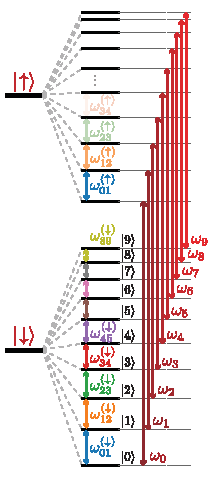
\includegraphics{chapter2/figures/energy_levels_ninehalf.pdf}
    \caption[Energy level diagram of an Er3+ coupled to a nuclear spin-9/2]{Energy level diagram of an Er3+ coupled to a nuclear spin-9/2. EPR-allowed transitions are depicted as red arrows while nuclear spin transitions are shown as multicolored arrows. \red{notation of electron spin}}
    \labfig{energy_levels_ninehalf}
\end{marginfigure}

In chapter \red{refch} we report the observation of an \Er electron-spin coupled to a $I=9/2$ nuclear spin. Through spectroscopic analysis of the nuclear spin transitions, we identify the nature of the spin as a \Nb. The Hamiltonian for this system extends the \W--\Er model by including the nuclear electric quadrupole interaction, which is present for all nuclei with $I\ge 1$ (see \refsec{electric_quadrupole}). In this section we describe the Hamiltonian of the system, the resulting energy levels and the transition frequencies at first order approximation. In addirtionWe note that the gyromagnetic factor of \Nb is approximately an order of magnitude larger than \W, which result in a larger separation of the nuclear spin levels. 

The Hamiltonian of the \Nb-\Er system is

\begin{equation}
    \cH{}/\hbar = \omega_S \hat{S}_z + \omega_I \hat{I}_z + A_\parallel \hat{S}_z \hat{I}_z + A_\perp \hat{S}_z \hat{I}_x + \hat{\mathbf{I}} \cdot \bar{\bar{Q}} \cdot \hat{\mathbf{I}}.
   \label{eq:hamiltonian_spin_9o2}
\end{equation}

This Hamiltonian yields twenty energy levels, illustrated in \reffig{energy_levels_ninehalf}. Under the secular approximation the electron spin projection $m_S$ remains a good quantum number, so the full manifold effectively separates into two submanifolds $(m_S = \Uparrow, \Downarrow)$ of ten nuclear-spin levels each. By contrast, the nuclear-spin states are influenced by both the hyperfine coupling and the electric quadrupole interaction, which mix states with different $m_I$. It is useful to distinguish three regimes according to the relative strength of the nuclear Zeeman and quadrupole terms:

\begin{itemize}
    \item Weak-quadrupole regime: \(\omega_I \gg \|\bar{\bar{Q}}\|\). The quadrupole interaction can be treated perturbatively and nuclear eigenstates are approximately the Zeeman states \(\ket{I,m_I}\), split by small quadrupolar corrections.
    \item Strong-quadrupole regime: \(\omega_I \ll \|\bar{\bar{Q}}\|\). Quadrupole effects dominate and the Zeeman term is the perturbation; nuclear eigenstates are then close to the quadrupole principal-axis eigenstates.
    \item Intermediate regime: \(\omega_I \sim \|\bar{\bar{Q}}\|\). Both interactions are significant and need to be treated simultaneously. The energy levels of the system are not trivial
\end{itemize}

In Chapter \red{refch} the measured system lies between the weak- and intermediate-quadrupole regimes: the nuclear Zeeman term still dominates, so most eigenstates are well approximated by the magnetic quantum number $m_I$, but the quadrupolar interaction produces noticeable mixing for the lower-frequency levels. We label the nuclear eigenstates by \(n\in\{0,1,\dots,9\}\) in order of increasing energy (see \reffig{energy_levels_ninehalf}), which at first-order approximation to $m_I = 9/2 - n$. Consequently, the ten EPR-allowed transitions, labeled as $\omega_n$ for each nuclear spin state, have frequencies given by

\begin{equation}
    \omega_n \approx \omega_S + m_I A_\parallel = \omega_S + \left(\tfrac{9}{2}-n\right) A_\parallel,
\end{equation}

although small corrections to these frequencies arise from second-order quadrupolar shifts, but are considerably smaller than the linewidth of the transitions and can be disregarded.

Our measurements reveal that the quadrupole's principal axis $\mathcal{P}_3$ is approximately parallel to the crystalline $c$-axis. Therefore, the other two axes must lie in the $(a,b)$-plane and make an arbitrary angle $\alpha_Q$ with respect to the crystalline $a$-axis. Because $B_0$ is nearly parallel to $c$, we adopt the approximation\sidenote{In the nuclear-spin operator frame the $z$-axis is defined by the external field $B_0$ (approximately parallel to the crystal $c$-axis). The $x$- and $y$-axes therefore lie in the $(a,b)$-plane, and the x-axis makes an angle $\alpha_\text{hf}$ with the crystalline $a$-axis; $\alpha_\text{hf}$ depends on the field orientation and the hyperfine tensor.} $z \parallel c \parallel \mathcal{P}_3$. Under this approximation the quadrupole Hamiltonian (given by Eq. \ref{eq:quadrupole_ppaxis}) can be written as

\begin{align}
\begin{split}
        \cH{Q}/\hbar &= \frac{\omega_Q'}{6} \left[3\hat{I}_{z}^2 + \frac{\eta'}{2}(e^{-2i\alpha}\hat{I}_+^2-e^{2i\alpha}\hat{I}_{-}^2)\right] \\
        \omega_Q' &= -\frac{\eta+1}{2} \, \omega_Q, \\ 
        \eta' &= \frac{\eta-3}{1+\eta}.
\end{split}
\end{align} 

where $\alpha=\alpha_\text{hf} - \alpha_Q$. Therefore, the Hamiltonian of the system can be approximated by 

\begin{align}
\begin{split}
       \cH{}/\hbar &= \omega_S \hat{S}_z + \omega_I \hat{I}_z + A_\parallel \hat{S}_z \hat{I}_z + A_\perp \hat{S}_z \hat{I}_x + \\ 
        &+ \frac{\omega_Q'}{6} \left[3\hat{I}_{z}^2 + \frac{\eta'}{2}(e^{-2i\alpha}\hat{I}_+^2-e^{2i\alpha}\hat{I}_{-}^2)\right].
\end{split}
\end{align}

 \red{nuclear spin transitions}